\documentclass[11pt]{article}
\usepackage[margin=2cm]{geometry}
\usepackage{enumitem} 
\usepackage{amsmath} 
\usepackage{amsfonts}
\usepackage{graphicx}
\usepackage{float} 
\newcommand{\R}[0]{\mathbb{R}}

% relativity commands
\newcommand{\srmetric}[0]{\eta_{\mu \nu}}
\newcommand{\grmetric}[0]{g_{\mu \nu}}
\newcommand{\riemanntensor}[0]{\tensor{R}{^\rho_{\sigma \mu \nu}}}

% physics packages 
\usepackage{tensor}

% physics shortcuts 
\newcommand{\kltensor}[0]{\tensor{T}{^{\mu_1 ... \mu_k}}_{\nu_1 ... \nu_l}}
\newcommand{\christoffel}[0]{\tensor{\Gamma}{^\rho_{\mu \nu}}}


% hyper-ref commands
\usepackage{hyperref}
\hypersetup{
    colorlinks,
    citecolor=black,
    filecolor=black,
    linkcolor=black,
    urlcolor=black
}

% math commands
\usepackage{amsthm}
\theoremstyle{definition}
\newtheorem{definition}{Definition}[section]

% tensor products
\usepackage{xparse}

\NewDocumentCommand{\tens}{t_}
 {%
  \IfBooleanTF{#1}
   {\tensop}
   {\otimes}%
 }

\setlist[enumerate]{itemsep=0mm}
\setenumerate{label=(\arabic*)}
\begin{document}
\begin{center}
	\textbf{PHYS 514: General Relativity Lecture Notes} \\
	\textbf{Shereen Elaidi}
\end{center}
\tableofcontents

\section{Lecture 1: 7 January 2020}
\emph{What is GR?} GR is the modern theory of classical gravity that incorporates the effects of special relativity. The basic idea is the following: gravity is a force. Most forces are described by fields. \emph{What are fields}? We have the following examples of fields: 
\begin{enumerate}[noitemsep]
	\item The Newtonian gravitational Potential, \( \Phi \). 
	\item For electromagnetism, we have the electromagnetic fields \(  E \) and \( B \). 
\end{enumerate}
We call such a theory a \textbf{field theory}. A classical field theory has two ingredients that make up a theory of forces described by fields: 
\begin{enumerate}[noitemsep]
	\item \textbf{A field equation}: an equation of motion which tells us exactly how the field is determined by some set of forces. This is typically a 2nd order ODE. For example: 
	\begin{enumerate}[noitemsep]
		\item The field equation for Newtonian gravity is \( \nabla^2 \Phi = 4 \pi G \rho \). 
		\item The field equations for E\&M are Maxwell's equations. 
	\end{enumerate}
	\item \textbf{Force Law:} an equation which determines how objects move in the presence of a field. For example: 
	\begin{enumerate}[noitemsep]
		\item For Newtonian gravity, this is \( F = ma = m \nabla \Phi \).
		\item For E\&M, this is the Lorentz force law \( F = q(E + v \times B ) \).
	\end{enumerate}
\end{enumerate}
The fields are functions of points in space-time. We write them as \( \Phi(t,x) \) for the gravitational field or \( E(t,x) \) for the electric field. The force law tells us how the objects move, i.e., how they deviate from a straight line (\( a = 0 \) ). The modern perspective of GR is the following: it is not a field theory; it is something totally different-- gravity is not due to a field \( \Phi \) that is a function of space-time, but is instead a feature of space-time itself. Hence, we replace the \( \Phi \) with a ``metric tensor'' which describes the curvature / geometry of space-time. 
\newline
\newline
The field equation of GR determines how space-time curves in the presence of matter or energy. This field equation is a differential equation for the metric of space-time that helps us determine how space-time curves in the presence of matter. 
\newline
\newline
The force law is the geodesic equation, which tells us how objects move through curved space-time. In short, this means that objects travel on \textbf{geodesics}, which are as straight as possible given the curvature of space-time. For example, on a plane, the shortest way to travel between two points is simply a line. However, for a sphere, the curve that minimises distance is the arc of a great circle. 

\section{Lecture 2: 12 January 2021} 
Space time is a set of points at which events could take place, which can be parameterized in a smooth manner by a coordinate system, such as cartesian coordinates (t, x). We call points in space-time \textbf{events}. Physics should be independent of the coordinate system used. 
\newline 
\newline 
In Newtonian physics, for two points \( (t_1, x_1) \) and \( (t_2, x_2) \), we can define the time-separation and spatial separations:
\begin{align*}
	\Delta t & = t_2 - t_1, \\
	\Delta x & = \sqrt{(x_2-x_1)^2}.
\end{align*}
These two quantities have independent meaning and make sense in Newtonian physics (this is called the principle of general covariance). In SR, there is no separate notion of time and space (time separation/distance) between two events. In other words, \( \Delta t \) and \( \Delta x \) do not make sense independently. These depend on the frame of reference in which they are measured. But, there is a notion of an ``invariant interval'' between two events. Given two events, 
\begin{align*}
	\Delta s^2 & = -c^2 \Delta t^2 + \Delta x^2 \\
			& = - \Delta t^2 + \Delta x^2 \text{ (units where \( c = 1 \) ) }
\end{align*}
When we talk about space-time, it's useful to draw pictures. We'll plot pictures in space-time using a \textbf{space-time diagram}, with time running vertically. Curves of a fixed \( \Delta s \) trace out hyperbolae. We have that light-rays travel on \( 45 \) degree lines. We have three cases: 
\begin{enumerate}[noitemsep]
	\item \( \Delta s^2 = 0 \): these two points can be connected by a light ray. These pairs of events are called \textbf{null-separated} or \textbf{light-like separated}. 
	\item \( \Delta s^2 < 0 \): these points/events can be connected with a trajectory with a velocity less than \( c \). We call such events \textbf{time-like separated}. 
	\item \( \Delta s^2 > 0 \): these are points which cannot be connected as above. We call such events \textbf{space-like separated}.
\end{enumerate}
\textbf{Claim:} all of special relativity can be reduced to the following statement: 
\begin{quote}
	For two time-like separated events, the proper time \( \Delta \tau \) measured by an observer moving at a constant velocity between the events is given by:
	\begin{align*}
		( \Delta \tau ) ^2 = - ( \Delta s)^2.
	\end{align*}
\end{quote}
This reproduces various phenomena. For example, consider \textbf{time-dilation}. Using the above, we can deduce that the relative age difference between the two twins would be \( \frac{2 \Delta \tau}{\Delta t} =\sqrt{1-v^2} \). We see a similar result for \textbf{length contraction}: \( \frac{\Delta \tau^2}{t^2} = 1 - v^2 \). In our world, we have three spatial coordinates, and so the invariant interval takes the following form:
\begin{align*}
	\Delta s^2 = - \Delta t^2 + \Delta x_1^2 + \Delta x_2^2 + \Delta x_3^2. 
\end{align*}
To write this more compactly, we'll introduce a new notation. Let \( x^\mu = (t, x) \) where \( \mu = 0, 1, 2, 3 \). Then, we can write the invariant interval as: 
\begin{align}
	(\Delta s)^2 & = \sum_{\mu, \nu = 0}^3 g_{\mu \nu} \Delta x, 
\end{align}
where, 
\begin{align*}
	g_{\mu \nu} = \begin{bmatrix}
		-1 & 0 & 0 & 0 \\
		0 & 1 & 0 & 0 \\
		0 & 0 & 1 & 0 \\
		0 & 0 & 0 & 1
	\end{bmatrix}. 
\end{align*}
That matrix is the ``metric'' of flat space-time in cartesian coordinates. We can write things even more compactly by introducing \textbf{Einstein summation notation}:
\begin{align*}
	\Delta s^2 = g_{\mu \nu} \Delta x^\mu \Delta x^\nu. 
\end{align*}
We read this by knowing that repeated indices are summed. Since \( \mu \) and \( \nu \) range from 0 to 3, we will be summing the above from 0 to 3. 
\newline
\newline
You are familiar with Euclidean space \( \R^2 \) and \( \R^3 \). Minkowski space is denoted by \( \R^{3,1} \); this is just like \( \R^4 \) except we have a negative sign in the formula for the distance. This gives us a \textbf{Lorentzian space-time}. 


\section{Lecture 3: 14 January 2021}
\subsection{Special Relativity and the Equivalence Principle}
We left off last time with a reformulation of special relativity as the geometry of space-time. In particular, 
\begin{quote}
	The proper time \( \Delta \tau \) measured by an observer moving at a constant velocity between two points in space-time is given by the invariant interval \( \Delta s \): 
	\begin{align*}
		(\Delta \tau)^2 = - (\Delta s)^2, 
	\end{align*}
	where \( \Delta s^2 = - \Delta t^2 + (\Delta x)^2 \) in Cartesian coordinates. 
\end{quote}
Recalling that \( \Delta x^\mu = (\Delta t, \Delta x) \), we can write the above using the metric as: 
\begin{align*}
	\Delta s^2 = \eta_{\mu \nu} \Delta x^\mu \Delta x^\nu, 
\end{align*}
where the metric is given by the following matrix:
\begin{align*}
	\ \eta_{\mu \nu} = \begin{bmatrix}
		-1 & 0 & 0 & 0 \\
		0 & 1 & 0 & 0 \\
		0 & 0 & 1 & 0 \\
		0 & 0 & 0 & 1 
	\end{bmatrix}. 
\end{align*}
Now, we want to build up to the equivalence principle. This requires us to think about observers who are accelerating (basic idea of the equivalence principle). For us, accelerating means that observers are moving through a path in space-time which is not in a straight line. 
\newline
\newline
A general path through space-time is known as a \textbf{world-line}. It is parameterized by four functions. Let \( \lambda \) be our parameter which labels different points on the curve. Then:
\begin{align*}
	x^\mu(\lambda) = (t (\lambda), x^1(\lambda), x^2 (\lambda), x^3 (\lambda)). 
\end{align*}
\textbf{Q: How would you measure the proper time of an observer moving on this trajectory: \( \Delta \tau \)?}
The proper time \( \Delta \tau \) measured on an observer can be obtained by taking the following limiting process: break the curve down into small segments, approximate each segment by straight lines, then apply the formula from the previous lecture to proper time along a straight line. Then, take the limit as the length of each interval goes to zero. This gives us that the proper time along a path is \( \sqrt{-(\Delta s)^2 } \), where
\begin{align}
	\Delta s = \int \sqrt{- \left( \frac{dt}{d \lambda} \right)^2 + \left(  \frac{dx^1}{d \lambda} \right)^2 + \left(  \frac{dx^2}{d  \lambda} \right)^2 + \left(  \frac{dx^3}{d \lambda} \right)^2} d \lambda. 
\end{align}
Observe that the above is similar to the arc-length of a curve from calculus. Using the Einstein summation notation, we can write this more compactly as: 
\begin{align}
\Delta s= \int \sqrt{\srmetric \frac{\partial x^\mu}{\partial \lambda} \frac{\partial x^\nu}{\partial \lambda}} d \lambda. 	
\end{align}
We will write this as \( \Delta s= \int ds \), where \( ds \) is an infinitesimal interval of space-time. We call it the \textbf{line-element of ST in GR}: 
\begin{align*}
	ds^2 = \srmetric dx^\mu dx^\nu 
\end{align*}
which we got by cancelling the \( d \lambda \) in the above. Now, special relativity is the statement that ``line element'' is given by
\begin{align*}
	ds^2 = \srmetric dx^\mu dx^\nu  \text{ with } \srmetric = \begin{bmatrix}
		-1 & 0 & 0 & 0 \\
		0 & 1 & 0 & 0 \\
		0 & 0 & 1 & 0 \\
		0 & 0 & 0 & 1
	\end{bmatrix}.
\end{align*}
GR is a very simple modification of the above statement; GR is the statement that all the effects of gravity are packages in terms of the replacement of \( \srmetric \) by \( \grmetric(x) \); the components depend on the coordinates themselves. We call this the ``metric of curved space-time.'' \( \srmetric \) is parameterized by 16 functions of \( x \). Hence, to summarise, every statement of ST goes to GR with the proviso that 
\begin{align}
	ds^2 = \grmetric dx^\mu dx^\nu. 	
\end{align}
In GR, light rays still travel along null trajectories, but the null trajectory is defined as \( ds = 0 \) rather than \( \Delta s = 0 \) as previously. Similarly, time-like trajectories (trajectories which massive objects travel along) has \( (ds)^2 < 0 \) for every point along the trajectory. The proper time measured by an observer who travels along a wordline \( x^\mu(\lambda) \) is again given by: 
\begin{align}
	\Delta \tau^2 = - \Delta s^2, 	
\end{align}
where \( \Delta s = \int ds \) where \( ds \) is given by:
\begin{align}
	\Delta s = \int \sqrt{\grmetric \frac{dx^\mu}{d \lambda} \frac{dx^\nu}{d \lambda}} d \lambda. 	
\end{align}

With this geometric formulation, general relativity is a nearly trivial modification of special relativity. Just replace \( \srmetric \) with \( \grmetric \). We still need some dynamical principle (this will be Einstein's field equations) and we need some mathematical tools. For example, the above gives us time dilation, which then give us phenomena such as red shift in cosmology and event horizons for black holes. 

\subsection{Why GR is a simple modification of SR (Equivalence Principle)}
The equivalence principle starts with a very simple but powerful observation about gravity. In Newtonian gravity, the way that you describe dynamics is by determining force. Let \( m_i \) be the inertial mass of an object and let \( m_g \) be the gravitational mass of an object. Let \( \Phi \) be the gravitational potential. Then, 
\begin{align*}
	F & = m_i a \\
	& = - m_g \nabla \Phi. 
\end{align*}
In principle, \( m_i \) may not be equal to \( m_g \). But, it is an \emph{experimental fact} that for every object that we know, \( m_i = m_g \). You can cancel them out and get the first \textbf{equivalence principle}: 
\begin{align} 
	\boxed{ a = - \Delta \Phi  } 
\end{align} 
for all objects, independent of their mass (think of the Leaning tower of Pisa experiment or the feather dropping experiments from space). Note that it is possible that we could discover a new form of matter for which this is not true, in which case we would need to modify GR to deal with that. The above implies that in the presence of a gravitational potential, there is a preferred set of trajectories which any freely-falling object would prefer. These trajectories are the solutions of \( a = - \Delta \Phi \). We call those trajectories \textbf{inertial trajectories}. 
\newline
\newline
Consider a small region of space-time where \( \nabla \Phi \) is approximately constant. Call that constant \( - a_0 \). The basic idea of the \textbf{Weak Equivalence Principle} is the following: 
\begin{quote}
	In this very small region, the effects of gravity are \emph{indistinguishable} from the effects of being in a constantly accelerating reference frame. 
\end{quote}
We can see this via a thought experiment. Consider two labs: one situated on Earth, and another attached to the end of a rocket in space which is accelerating with \( a_0 = g \). The EOM of an object in the first lab is \( \ddot{x} = -g \). The EOM of an object in the second lab would be \( x' = x- \frac{1}{2} gt^2 \), i.e., \( \ddot{x'} = -g \). This means that if you were to do experiments in these labs, there is no way to tell which scenario that you are in, i.e., the laws are the same. We call forces which arise due to acceleration \textbf{fictitious forces}. 
\newline
\newline
The equivalence principle is the statement that in a very small area, the effects of gravity are indistinguishable from a fictitious force due to acceleration. In this case, the metric of flat space-time (Minkowski space) will no longer be constant when written in terms of accelerating coordinates, which then gives us that the effects of gravity can be captured by changes in the metric. 
\newline
\newline
Once \( \Delta \Phi \) is no longer approximately constant, i.e., when we are no longer in a region of space-time which is small, we cannot just think of gravity in terms of acceleration (fictitious forces). For example, in a very lab due to tidal forces, we can use experiments to tell if there is varying gravitational potential present; this cannot be mimicked by a constantly accelerating reference frame.
\newline
\newline
Let's conclude by reformulating the EP (Equivalence Principle) a bit: 
\begin{quote}
	\textbf{Einstein Equivalence Principle}: in a sufficiently small region of space-time, the laws of physics reduce to those of SR. In other words, space-time \emph{locally} looks like Minkowski space \( \R^{3,1} \). 
\end{quote}
We'll spend the next few weeks unpacking the above statement. There's also a V2 of the EEP: 
\begin{quote}
	\textbf{EEP'}: for any point \( x_0^\mu \), there is a coordinate system such that the line element takes the form of that in SR near \( x_0^\mu \). Mathematically: 
	\begin{align*}
		ds^2 = \srmetric dx^\mu dx^\nu + O(x-x_0^\mu), 
	\end{align*}
	where \( O(x-x_0^\mu) \) represents the extent to which gravity is not a fictitious force. 
\end{quote}


\section{Lecture 4: 19 January 2020}
\subsection{Manifolds}
Space-time locally ``looks like'' Minkowski space \( \R^{3,1} \). On larger scales, gravity cannot just be regarded as a fictitious force. It's in the sense that a sphere locally looks like flat space. Precisely, this is the statement that ST is a four-dimensional pseudo-Riemannian \textbf{manifold}. We say that A \( D \)-dimensional \textbf{manifold} \( M \) is a set of points that can be labelled by coordinate systems in a smooth way. 
\newline
\newline
Precisely, a coordinate system is a set of \( d \) functions \( x^i \) which label different points in some region \( U \subseteq M \) in a unique way. Mathematically, this is expressed as:
\begin{align*}
	x^i: \mathcal{U} \rightarrow \R^d, \hspace{1cm} i = 1, ..., D.
\end{align*}
The region \( \mathcal{U} \) which these coordinates label uniquely is called a \textbf{patch} or \textbf{coordinate patch} of the manifold which is `` covered'' by the \( x^i \). A \textbf{global coordinate system} is one which covers all of \( M \). Generally, there are many coordinate systems which may cover some patch \( \mathcal{U} \) of \( M \). 
\newline
\newline
\textbf{E.g.:} \( x^i \) and \( x^{i'} \) are two different ways of labelling points in \( \mathcal{U} \). Then, we can talk about the coordinate transformation or a change of coordinates between \( x^i \) and \( x^{i'} \). These functions will be parameterized and \( C^\infty \). 
\begin{align*}
	x^i(x^{i'}) \text{ or } x^{i'}(x^i).
\end{align*}
If the coordinates \( x^i \) and \( x^{i'} \) uniquely, label points in some region \( \mathcal{U} \), then the Jacobian matrix
\begin{align*}
	\frac{\partial x^i}{\partial x^{i'}} = \frac{\partial x^{i}}{\partial x^{j'}}, 
\end{align*}
is invertible (each index runs from \(1, ...D \)). This describes the components of a \( D \times D \) matrix. If it's invertible, then we have that \( \text{det}\left(\frac{dx^i}{dx^j}  \right) \neq 0 \). If the determinant is zero, then one of the coordinate system has become degenerate in some way in the sense that it no longer labels points in a unique way. Hence, the coordinate system becomes singular. 
\newline
\newline
For example, the plane \( \R^2 \) describes a two-dimensional manifold. Two coordinate systems on this manifold are the cartesian coordinates \( (x,y) \) (global coordinates) and polar coordinates \( (r, \theta) \). They are related by a chance of coordinates: 
\begin{align*}
	x^i & = (x^1, x^2)  = (x,y), \\
	x^{i'} & = (x^{1'}. x^{2'} )  = (r, \theta).
\end{align*}
Then, the coordinate transformations arse given by: 
\begin{align*}
	x^{i}(x^{i'}): x = r \cos \theta,\ y = r \sin \theta
\end{align*}
and the inverse transformation is given by: 
\begin{align*}
	x^{i'}(x^{i}): r = \sqrt{x^2 + y^2},\ \theta = \arctan (y/x). 
\end{align*} 
Hence, the Jacobian matrix is given by: 
\begin{align*}
	\left( \frac{\partial x^i}{\partial x^{j'}} \right) & = \begin{bmatrix}
		 \cos \theta & \sin \theta \\
		 - r \sin \theta & r \cos \theta 
	\end{bmatrix}
\end{align*}
We have that \( \text{det}(\text{jac}) = r \cos^2 \theta + r \sin^2 \theta = r \), which is non-zero only if \( r \neq 0 \).
\newline
\newline
When describing space-time, we usually use a spatial notation for the coordinates: 
\begin{align*}
	x^\mu, \mu = 0, ..., 3. 
\end{align*}
Having greek indices mean that we are describing space-time; having Roman indices mean that we are describing a Euclidean manifold. For example: 
\begin{align*}
	x^\mu = (t, x) \text{ of } \R^{3,1} \text{ is an example of a coordinate system on a space-time.} 
\end{align*} 
\textbf{Most important sentence of this lecture: our goal is to write the laws of physics in such a way that any physical prediction made by these laws is independent of the choice of coordinate systems that we use to write the law.} For example, we had the same laws in Newtonian physics for both polar and cartesian coordinates. We give this goal the following name: \textbf{Principle of General Covariance}. 
\newline
\newline
E.g., in previous lectures we met the line element \( ds^2 = \eta_{\mu \nu} dx^\mu dx^\nu \).  Under some change of coordinates \( x^\mu \rightarrow x^{\mu'}(x^\mu) \), we have that the line element transforms by multiplication by the Jacobian matrix: 
\begin{align*}
	dx^\mu = \left( \frac{\partial x^\mu}{\partial x^\nu} \right) dx^{\nu'}, 
\end{align*}
What this is saying is the following: if I displaced \( \nu' \) by some infinitesimal amount, and asked how much \( \mu \) changed, then the above equation (basically thanks to the chain rule), will answer that question for us. This becomes clear with an example: 
\newline
\newline
\textbf{E.g.:} set \( x = r \cos \theta, y = r \sin \theta \). Then, 
\begin{align*}
	dx & = \cos \theta r -  r \sin \theta d \theta, \\
	dy & = \sin \theta dr + r \cos \theta d \theta. 
\end{align*}
How does the line element transform? We apply the formula:
\begin{align*}
	ds^2 & = \srmetric dx^\mu dx^\nu \\
		& = \left( \frac{\partial x^\mu}{\partial x^{\mu'}} dx^{\mu'} \right) \left( \frac{\partial x^\nu}{\partial x^{\nu'}} dx^{\nu'} \right) \srmetric \\
		& = g_{\mu' \nu'}dx^{\mu'} dx^{\nu'}, 
\end{align*}
where 
\begin{align*}
	g_{\mu' nu'} = \srmetric \frac{\partial x^\mu}{\partial x^{\mu'}} \frac{\partial x^\nu}{\partial x^{\nu'}}. 
\end{align*}
In other words, the metric transforms as: 
\begin{align*}
	\srmetric \rightarrow g_{\mu' \nu'} = \srmetric \frac{\partial x^\mu}{\partial x^{\mu'}} \frac{\partial x^\nu}{\partial x^{\nu'}}. 
\end{align*}
\textbf{E.g.:} the line element of flat space \( \R^2 \) is the thing that we use to measure distances: 
\begin{align*}
	ds^2 = dx^2 + dy^2. 
\end{align*}
In polar coordinates, this becomes: 
\begin{align*}
	ds^2 & = dx^2 + dy^2 \\
	& = ( \cos \theta dr - r \sin \theta d \theta)^2 + ( \sin \theta dr + r \cos \theta d \theta)^2 \\
	& = dr^2 + r^2 d \theta 
\end{align*}
\section{Lecture 5: 21 January 2021}
\subsection{Tensors}
Our goal is to formulate the laws of physics such that things are independent of the coordinate systems in which we use to measure them. This goal is called the \textbf{Principle of Covariance}. This goal underlies everything that we will be discussing today. To tackle this goal, we will need to understand how quantities transform under coordinate transformations. 
\newline
\newline
To that end, consider a D-dimensional manifold \( M \). A patch \( M \) can be described by multiple different coordinate systems; say, \( x^\mu \) and \( x^{\mu'} \). The simples object that can transform is a \textbf{scalar/scalar function}. 
\newline
\newline
A \textbf{scalar function} \( f \) is an assignment of a number to each point on a manifold \( M \) which is \emph{independent} of the coordinates. For example: 
\begin{align*}
	& f(x^\mu) \text{ in } x^\mu \text{ coordinates.} \\
	& f(x^{\mu'}) \text{ in } x^{\mu'} \text{ coordinates}  = f(x^{\mu'}(x^\mu)) \text{ in } x^{\mu'} \text{ coordinates.} 
\end{align*}
We say that \( f \) is invariant under the change of coordinates \( x^\mu \rightarrow x^{\mu'} = x^{\mu'}(x^\mu) \). A scalar function is called a \textbf{(0,0)-tensor}. 
\newline
\newline
A \textbf{vector} is a set of \( D \) functions \( V^\mu \) (in each coordinate system) which transforms under changes of coordinates in a particular way: 
\begin{align*}
	& V^\mu (x^\mu)  \text{ in } x^\mu \text{ coordinates.} \\
	& V^{\mu'} (x^{\mu'}) = \frac{\partial x^{\mu'}}{\partial x^\mu} V^\mu (x^{\mu'}(x^\mu)). 
\end{align*}
This is known as a \textbf{contravariant} vector or a \( (1,0) \)-tensor. This is a generalisation of the usual idea of a vector in multivariable calculus. For example, consider \( \R^3 \), and let \( v \) be a vector. We can represent \( v \) in a specific coordinate system with the following components: \( v = (v^1, v^2, v^3) \). If we were to rotate the axes, then we can express the rotation with a rotation matrix \( R \): 
\begin{align*}
	\begin{bmatrix}
		x' \\
		y' \\
		z' \\
	\end{bmatrix} = R \begin{bmatrix}
		x \\
		y \\
		z \\
	\end{bmatrix}
\end{align*}
The components of \( v \) in this new coordinate system would accordingly change:
\begin{align*}
	\begin{bmatrix}
		v^{1'} \\
		v^{2'} \\
		v^{3'} \\
	\end{bmatrix} = \begin{bmatrix}
		R^{1}_2 & R_2^1 & R_3^1 \\
		\vdots & \ddots & \vdots \\
		R_1^r & \hdots & R_3^3
	\end{bmatrix} \begin{bmatrix}
		v^1 \\
		v^2 \\
		v^3
	\end{bmatrix}
\end{align*}
The \emph{components} of the vector will transform by the multiplication of the transformation matrix. To see how this exactly works out, let \( v^i \) be the components of \( v \) in the unprimed coordinate frame, and let \( v^{i'} \) be the components in the un-primed frame. Using index multiplication, we will discover that Einstein summation notation is basically repackaging matrix multiplication:
\begin{align*}
	v^{i'} = R^{i'}_j v^j, 
\end{align*} 
that is, \( R \) is simply the Jacobian:
\begin{align*}
	R^{i'}_j = \frac{\partial x^{i'}}{\partial x^j}. 
\end{align*}
So, our definition of a vector is simply an object that obeys the following transformation rule: \( v^{\mu'} = \frac{\partial x^{\mu'}}{\partial x^\mu} v^\mu \); it's just a generalisation from vector calculus which accommodates more interesting and non-linear coordinate transformations. This is interesting to us if we think about Einstein's Equivalence Principle. Even tho the components of our vecttor, 
\begin{align*}
	v^\mu & = \begin{bmatrix}
		v^0 \\
		\vdots \\
		v^3 
	\end{bmatrix} 
\end{align*} 
will look different in different coordinate systems, a vector should be regarded as a \textbf{geometric object} with \emph{coordinate-independent meaning}. A typical example is as follows: consider a world line \( x^\mu(\lambda) \) which is moving through the manifold. The points on this curve are parameterised by some variable \( \lambda \). We can then define the vector \( v^\mu := \frac{ \partial x^\mu }{ \partial \lambda} \); this is the tangent vector to the world-line. 
\newline
\newline
\textbf{Why is this a vector in the sense of tensor calculus?} This is a vector because of the chain rule; the chain rule says that in the new coordinates \( x^{\mu'}(x^\mu) \): 
\begin{align*}
	v^{\mu'} = \frac{\partial x^{\mu'}}{\partial \lambda} = \left( \frac{\partial x^{\mu'}}{\partial x^\mu} \right) \frac{\partial x^\mu}{\partial \lambda }, 
\end{align*}
where \( \left( \frac{\partial x^{\mu'}}{\partial x^\mu} \right) \) is the Jacobian matrix.  We can consider the set of all tangent vectors -- the \textbf{tangent space}, denoted \( T_p(M) \) -- is the set of all tangent vectors attached to a point \( p \) of \( M \). This is a vector space. A tangent vector is an example of a vector that is defined for each point on a curve. A vector attached to each point in \( M \) is called a \textbf{vector field}; in this class, if we talk about a vector, we mean a VECTOR FIELD.
\newline
\newline
We can also use our vectors to define differential operators. Given a scalar \( f \) and a vector \( v^\mu (x^\mu) \), we can define the \textbf{differential operator} \( v \) by:
\begin{align*}
	vf := v^\mu \frac{\partial }{\partial x^\mu} f = v^\mu \partial_\mu f = v^\mu f_{ , \mu}. 
\end{align*}
This is precisely the directional derivative in the direction \( v \). For this to be well-defined, \( vf \) must be a scalar. Indeed, we have that it is a scalar by the chain rule. 
\begin{align*}
	vf = v^{\mu'} \frac{\partial }{\partial x^{\mu'}} f = v^\mu \left( \frac{\partial x^{\mu'}}{\partial x^\mu} \right) \left( \frac{\partial x^\nu}{\partial x^{\mu'}} \right) \frac{\partial}{\partial x^\nu}f. 
\end{align*}
In particular, by the chain rule, 
\begin{align*}
	\frac{\partial x^{\mu'}}{\partial x^\mu} \frac{\partial x^\nu}{\partial x^{\mu'}} = \frac{\partial x^\nu}{\partial x^\mu}. 
\end{align*}
Since the product of the two Jacobians, 
\begin{align*}
	J = \begin{bmatrix}
		\frac{\partial x^{1'}}{\partial x^1} & \hdots & \frac{\partial x^{D'}}{\partial x^1} \\
		\vdots  & & \vdots \\
		\frac{\partial x^{1'}}{\partial x^D} & \hdots & \frac{\partial x^{D'}}{\partial x^D}
	\end{bmatrix}
\end{align*}
and 
\begin{align*}
	\hat{J} = \begin{bmatrix}
		\frac{\partial x^{1}}{\partial x^{1'}} & \hdots & \frac{\partial x^{D}}{\partial x^{1'}} \\
		\vdots  & & \vdots \\
		\frac{\partial x^{1}}{\partial x^{D'}} & \hdots & \frac{\partial x^{D}}{\partial x^{D'}}
	\end{bmatrix}
\end{align*}
gives us the identity, that means: 
\begin{align*}
	vf = v^\mu \delta_\mu^\nu \frac{\partial f }{\partial v} = v^\mu \frac{\partial}{\partial x^\mu} f.
\end{align*}
This verifies that the differential operator \( v = v^\mu \partial_\mu \) takes scalars to scalars. We call this the \textbf{directional derivative in the direction of \( v \)}. If we had some scalar function, 
\begin{align*}
	f(x^\mu(\lambda)) = f(\lambda), 
\end{align*}
then we can intepret the directional derivative as: 
\begin{align*}
	\frac{df}{d \lambda} = \frac{\partial x^\mu}{\partial \lambda} \frac{\partial f}{\partial x^\mu} = v^\mu \frac{\partial}{\partial x^\mu}f.
\end{align*}
The geometric interpretation of this is as follows: this operator takes a derivative along the curve to which \( v \) is a tangent vector. Sometimes, we think of this \( \partial_\mu \) as a ``basis'' for the set of vector in the same sense that the \( e_i \) form a standard basis of \( \R^n \): 
\begin{align*}
	v = v^\mu \partial_\mu
\end{align*}

\section{Lecture 6: Tensors 26 January 2021}
A tensor is a generalisation to the manifold the idea of a vector or a matrix. We already met other tensors before: 
\begin{itemize}[noitemsep]
	\item A \textbf{scalar}, or a \( (0,0) \)-tensor, is a number for each point in a manifold \( M \). It is of the form of \( f(x^\mu) \).
	\item A \textbf{vector}, or a \( (1,0) \)-tensor, is a collection of \( D \) functions of the coordinates which transforms as:
	\begin{align*}
		v^\mu \rightarrow v^{\mu'} = \frac{\partial x^{\mu'}}{\partial x^{\mu}} v^{\mu}.
	\end{align*}
	We call the matrix \( \frac{\partial x^{\mu'}}{\partial x^{\mu}}  \) the Jacobian matrix. We can write this more familiarly as a Jacobian matrix: 
	\begin{align*}
		J \cdot v, 
	\end{align*}
	where \( v \) is a column vector. 
\end{itemize} 
These are the two tensors which we have met so far. We can represent a vector \( v^{\mu} \) in a \emph{coordinate-independent way} as a differential operator which takes scalars to tensors: 
\begin{align*}
	v = v^\mu \frac{\partial }{\partial x^\mu}, 
\end{align*}
where \( \mu \) is summed over according to the Einstein summation notation. 
\begin{enumerate}[noitemsep]
	\item A \textbf{one-form} is a set of \( D \) functions of the coordinates which transform as: 
	\begin{align*}
		\omega_\mu \rightarrow \omega_{\mu'} = \frac{\partial x^\mu}{\partial x^{\mu'}} \omega_\mu.
	\end{align*}
	Note that \( \frac{\partial x^\mu}{\partial x^{\mu'}} \) is the \emph{inverse} of the Jacobian. A one form looks similar to a vector. It is known as a \textbf{covariant vector}, or a \( (0,1) \)-tensor. Note that a one-form has a LOWER index whereas a vector has an UPPER index. 
\end{enumerate}
This is useful because if we have a one form \( \omega_\mu \) and a vector \( v^\mu \), then we can combine them to make a scalar. To see why, let's \textbf{contract} them together:
\begin{align*}
	v^\mu \omega_\mu \rightarrow v^{\mu'}\omega_{\mu'} & = \left( v^{\mu'} \frac{\partial x^{\mu'}}{\partial x^{\mu}} \right) \left( \frac{\partial x^{\nu}}{\partial x^{\nu'}} \omega_{\nu} \right) \\
	& = v^{\mu} \left(\frac{\partial x^{\mu'}}{\partial x^{\mu}} \frac{\partial x^{\nu}}{\partial x^{\mu}}  \right) \omega_{\nu}  \\
	& = v^{\mu} \delta_\mu^\nu \omega_\nu  \text{ (by the chain rule) } \\
	& = v^{\mu}\omega_{\mu}.
\end{align*} 
This shows that a vector and a one-form get combined together to make a scalar.  Formally, we can think of a one-form \( \omega_\mu \) as defining a map from vectors to numbers. We see one-forms referred to as \textbf{dual vectors} which live in a \textbf{dual tangent space}, \( T_p^*(M) \). You've encountered one-forms before. In linear algebra, we usually represent vectors as column vectors and one-forms as row vectors. 
\begin{align*}
	\omega_\mu = \begin{bmatrix}
		\omega_1 & \cdots & \omega_d 
	\end{bmatrix} \hspace{0.5cm} v^\mu = \begin{bmatrix}
		v^1 \\
		\vdots \\
		v^d 
	\end{bmatrix}. 
\end{align*}
The scalar you would have formed from these two objects is the dot product: 
\begin{align*}
	\omega_\mu v^\mu = \begin{bmatrix}
		\omega_1 & \cdots & \omega_d 
	\end{bmatrix} \begin{bmatrix}
		v^1 \\
		\vdots \\
		v^d 
	\end{bmatrix}. 
\end{align*}
The location of an index -- namely, if it's an upper index or a lower index -- tells us how an object transforms. When we set an upper and a lower index equal to each other and sum over them, we say that we are \textbf{contracting the indices}. 
\begin{align*}
	\omega_\mu v^\nu \rightarrow \omega_\mu v^\mu.
\end{align*}
Now consider a scalar \( f \). Then, we can define a one-form whose components are just the derivatives of \( f \) in a given coordinate system:
\begin{align*}
	\frac{\partial f}{\partial x^\mu} = \partial_\mu f.
\end{align*}
We can obtain the transformation rule for this by using the chain rule:
\begin{align*}
	\partial_\mu f \rightarrow \partial_{\mu'} f = \frac{\partial x^\mu}{\partial x^{\mu'}} \partial_\mu f, 
\end{align*}
which is indeed the multiplication rule that defines a one-form. Just as we write vectors in a basis-independent way as \( v = v^\mu \partial_\mu \), we can write one-forms in a basis-independent was as \( \omega = \omega_\mu dx^\mu \). We can think of the \( dx^\mu \) as infinitesimal displacements of the coordinate \( x^\mu \). They also form a basis of the cotangent space, and they transform as vectors: 
\begin{align*}
	\omega &  = \omega_\mu  dx^\mu \\
		   & = \left( \omega_{\mu'} \frac{\partial x^{\mu'}}{\partial x^{\mu}	} \right) \left( \frac{\partial x^{\mu}}{\partial x^{\nu'}} dx^{\nu'} \right) \\
		   & = \omega_{\mu'} dx^{\mu'}, 
\end{align*}
where the final equality follows from the chain rule. Since the notation is consistent, this proves that  \(  \omega_\mu  dx^\mu \) is a basis-independent representation of a one-form. There is a special notation for the one-form \( \partial_\mu f \): 
\begin{align*}
	df = \partial_\mu f dx^\mu. 
\end{align*}
If, for example, \( f = x^1 \), then this defines, by taking derivatives, the one-form whose components are the derivative of that function: 
\begin{align*}
	\partial_\mu (x^1) = (1, 0, ..., 0), 
\end{align*}
which is written as \( dx^1 \). Now we are ready to introduce the general definition of a tensor. 
\begin{definition}[Tensor]\label{def:tensor}
	A \((k,l)\)-\textbf{tensor}, \( \tensor{T}{^{\mu_1 ... \mu_k}}_{\nu_1 ... \nu_l} \), is a set of \( D^{k+l} \) functions which transform under coordinate transformations in a particular way: 
	\begin{align*}
		 \boxed{ \tensor{T}{^{\mu_1' ... \mu_k'}}_{\nu_1' ... \nu_l'} = \left( \frac{\partial x^{\mu_1'}}{\partial x^{\mu_1}} \right)  \hdots \left( \frac{\partial x^{\mu_k'}}{\partial x^{\mu_k}} \right) \left( \frac{\partial x^{\nu_1}}{\partial x^{\nu_1'}} \right) \hdots \left( \frac{\partial x^{\nu_l}}{\partial x^{\nu_l'}} \right) \kltensor }
	\end{align*}
\end{definition}
An easy way to remember Definition \ref{def:tensor} is to remember that this is the only way to ``balance the indices'' in a way that respects the Einstein summation convention: upper and lower indices are summed over. We call \( (k,l) \) the \textbf{rank of the tensor}, and \( k \) is the number of \textbf{contravariant indices} and \( l \) is the number of \textbf{covariant indices}. Crucial note: the order and placement of the indices in Definition \ref{def:tensor} matter! 
\newline
\newline
Sometimes you'll see people writing tensors in the coordinate-invariant way by contracting it with a bunch of partial derivatives and a bunch of one-forms that are multiplied together by using some cross product as a circle -- this is called a \textbf{tensor product}, but we'll leave that formal stuff to the mathematicians to deal with. 
\begin{align*}
	T = \kltensor \partial_{\mu_1} \tens \cdots \tens \partial_{\mu_k} \tens dx^{\nu_1} \tens \hdots \tens dx^{\nu_l}, 
\end{align*}
e.g., we can write a \( (0,2) \)-tensor with components \( g_{\mu \nu} \) as: 
\begin{align*}
	g & = g_{\mu \nu} dx^\mu \tens dx^{\nu} \\
	& = g_{\mu \nu} dx^{\mu} dx^{\nu}.
\end{align*}
Now, a few comments about tensors. There are three operations that we can do on tensors: 
\begin{enumerate}[noitemsep]
	\item \textbf{Add} together two tensors of the same rank to get another tensor of the same rank: 
	\begin{align*}
		\tensor{T}{^{\mu_1}_1^{...\mu_k}_{\nu_1 ... \nu_l}} + \tensor{T}{^{\mu_1}_2^{...\mu_k}_{\nu_1 ... \nu_l}} = \tensor{T}{^{\mu_1}_3^{...\mu_k}_{\nu_1 ... \nu_l}}. 
	\end{align*}
	\item \textbf{Multiply} a tensor with rank \( (k,l) \) with a tensor of rank \( (k', l') \) to get a tensor of rank \( (k+k', l+l') \): 
	\begin{align*}
		\kltensor \tensor{S}{^{\mu_{k+1} ... \mu_{k+k'}}_{\nu_{l+1}...\nu_{l+l'}}} \text{ is a tensor of rank \( (k+k', l+k') \).}
	\end{align*}
	\item Given a tensor of rank \( (k,l) \), we can \textbf{contract} an upper and a lower index together to get a tensor of rank \( (k-1, l-1) \): 
	\begin{align*}
		\tensor{T}{^{\mu_1 ... \alpha ... \mu_{k-1}}_{\nu_1 ... \alpha ... \nu_{l-1}}}.
	\end{align*}
	e.g., given a vector and a one-form, you can define a \( (1,1) \)-tensor \( v^\mu \omega_\nu \) with \( \mu \) and \( \nu \) separate indices, and \( v^\mu \omega_\mu \) as a scalar ( a \( (0,0) \)-tensor).
\end{enumerate}

\section{Lecture 7: 28 January 2021}
\subsection{Tensors and the Geometry of Space-Time}
From the operations on tensors introduced last class, we can build other operations. But first, let's define a math term. A \textbf{permutation} \( \sigma \) is a re-ordering of the numbers \( (1,..., l)  \rightarrow (1, ..., l ) \). A result from algebra tells us that \( \sigma \) is the product of pairwise interchanges. Using this notation, we can define two more operations on tensors: 
\begin{enumerate}[noitemsep]
	\item The \textbf{symmetrization} of a tensor makes it symmetric: 
	\begin{align*}
		T_{(\mu_1, ..., \mu_l)} = \frac{1}{l!} \sum_{\text{perms of } \sigma} \tensor{T}{_{\sigma(\mu_1) ... \sigma(\mu_l)}}. 
	\end{align*}
	\item The \textbf{anti-symmetrization} of a tensor makes it anti-symmetric: 
	\begin{align*}
		T_{[\mu_1 ... \mu_l]} = \frac{1}{l!} \sum_{\text{perms of } \sigma} \text{sgn}(\sigma) \tensor{T}{_{\sigma(\mu_1) ... \sigma(\mu_l)}}. 
	\end{align*}
\end{enumerate} 
For example: 
\begin{align*}
	T_{(\mu_1, \mu_2)} & = \frac{1}{2}( T_{\mu_1 \mu_2} + T_{\mu_2 \mu_1} ) \\
	T_{[\mu_1, \nu_2]} & = \frac{1}{2}( T_{\mu_1 \mu_2} - T_{\mu_2 \mu_1} ). 
\end{align*}
We can also do this procedure with upper indices or with only some fraction of the indices. E.g., we can consider something like this: 
\begin{align*}
	\tensor{T}{^{[\mu_1 \mu_2]}_{\nu_1 (\nu_2 \nu_3)}}. 
\end{align*}


\begin{definition}[(Anti)-Symmetric Tensor]\label{def:symmtens} 
	A \textbf{(anti)-symmetric tensor} is one which equals its (anti)-symmetrization. 
\end{definition}
\begin{itemize}[noitemsep]
	\item A symmetric tensor is unchanged when we permute two of its indices. 
	\item An anti-symmetric tensor will pick up a factor that is sgn(\(\sigma \)) when we interchange two of the indices. Hence, if two of the indices are equal for an anti-symmetric tensor, then the tensor is zero.
\end{itemize}

An anti-symmetric tensor of rank \( (0,n) \) is a \textbf{differential form of rank \( n \)}, e.g., an anti-symmetric \( (0,2) \)-tensor is a \(2\)-form. You've already met some tensors: 
\begin{align*}
	f & = (0,0)-\text{tensor.}  \\
	\partial_\mu f& = (0,1)-\text{tensor.} \\
	\frac{\partial x^\mu}{\partial \lambda} & = (1,0)-\text{tensor}  \text{ (tangent line of a world line).} \\
	\tensor{\delta}{^\mu_\nu} & = (1,1)-\text{tensor.} \\
	g_{\mu \nu} & \text{ a symmetric \((0,2)\)-tensor.} 
\end{align*}
\textbf{Why are we studying tensors?} The reason why is the Principle of General Covariance: the laws of physics should make predictions which should be \emph{independent} of the coordinate system that we use to write those laws. Hence, the laws of physics are TENSOR equations, i.e., every law of physics better take the form of 
\begin{align*}
	\kltensor = \tensor{S}{^{\mu_1 ... \mu_k}_{\nu_1 ... \nu_l}}
\end{align*}
in one reference frame, and 
\begin{align*}
	\tensor{T}{^{\mu_1' ... \mu_k'}_{\nu_1' ... \nu_l'}} = \tensor{S}{^{\mu_1' ... \mu_k'}_{\nu_1' ... \nu_l'}}, 
\end{align*}
in another reference frame, because of the tensor transformation rule (Jacobian matrices are invertible). For example, Maxwell's equations are tensor equations. 
\newline
\newline
We need to take derivatives of tensors now. We don't know how to do this in a \textbf{covariant manner}. Consider the only notion of differentiation that we have for now: 
\begin{align*}
	v^\mu \rightarrow \partial_\nu v^\mu \neq (1,1)-\text{tensor}, 
\end{align*}
This specifies a direction, and is not what we need. There is more than one way of formulating calculus on tensors. We'll be studying differential geometry / Riemannian geometry to do so. 
\newline
\newline
Recall the Einstein Equivalence Principle: the effect of gravity in a very small region of space-time is indistinguishable from an accelerating reference frame. Let's try to interpret this in a slightly more geometric point of view. \emph{Space-time is a manifold with a metric \( g_{\mu \nu}\) that is used to define the line-element}:
\begin{align*}
	ds^2 = g_{\mu \nu} dx^\mu dx^\nu, 
\end{align*}
\emph{such that for any point \( x_0^\mu \), there is a coordinate system such that}
\begin{align*}
	g_{\mu \nu} = \eta_{\mu \nu} + \text{ terms that vanish as } x^\mu_0 \rightarrow x_0^\mu, 
\end{align*}
\emph{i.e., we've Taylor expanded the metric about a point!} From this more geometric formulation of the Einstein Equivalence Principle, we find that \( \grmetric \) is a \((0,2)\)-tensor with three properties: 
\begin{enumerate}[noitemsep]
	\item \textbf{Symmetric}: \( \grmetric = g_{\nu \mu} \).
	\item \textbf{Invertible}: \( \text{det}(\grmetric) \neq 0 \). 
	\item \textbf{diagonalizablity}: \( g \) is diagonalizable with eigenvalues \( \lambda = -1, 1, 1, 1 \), i.e., there exists some basis where the metric can be expressed as \( \text{diag}(-1, 1, 1, 1) \). 
\end{enumerate}
These three properties are proven by noting that there exists some basis where \( \grmetric = \srmetric)\):
\begin{align*}
	\Rightarrow \grmetric = \left( \frac{\partial x^{\mu'}}{\partial x^{\mu}} \right) \left( \frac{\partial x^{\nu'}}{\partial x^{\nu}} \right) \eta_{\mu' \nu'} + ... , 
\end{align*}
i.e., in matrix notation:
\begin{align*}
	\grmetric = J^t \begin{bmatrix}
		-1 & 0 & 0 & 0 \\
		0 & 1 & 0 & 0 \\
		0 & 0 & 1 & 0 \\
		0 & 0 & 0 & 1
	\end{bmatrix} J. 
\end{align*}
The above properties are coordinate-invariant statements in the sense that if they are true in one coordinate system then they are true in every coordinate system. 
\newline
\newline
An invertible symmetric \( (0,2)\)-tensor is a \textbf{metric}. If the eigenvalues of the matrix are all positive, then we call it a \textbf{Riemannian metric}. Otherwise, we call it a \textbf{pseudo-Riemannian metric}. The number of positive and negative eigenvalues of \( \grmetric \) is called the \textbf{signature} of the metric. Using this new vocabulary, we can now say that in general relativity, space-time is a manifold with a pseudo-Riemannian metric of signature \( (-, +, +, +) \), or signature \( (1,3) \). 
\newline
\newline
\textbf{What can we do with this metric?}
\newline 
We can invert the metric. We'll denote the inverse of \( \grmetric \) as \( g^{\mu \nu} \). It is a symmetric \( (2,0)\)-tensor. Using the Einstein summation notation, we find: 
\begin{align*}
	g^{\mu \nu} g_{\nu \rho} & = \tensor{\delta}{^\mu_\rho}, \text{ or } \\
	g_{\mu \nu} g^{\nu \rho} & = \tensor{\delta}{^\rho_\mu} 
\end{align*}
\textbf{Conclusion:} the inverse of a metric is a tensor. We will use \( \grmetric \) and \( g^{\mu \nu} \) to raise and lower indices via Einstein summation notation. I.e., given a vector \( v^\mu \) we define a one-form \( v_\mu := \grmetric v^\nu \). Given a one-form \( \omega^\mu \), we define a vector \( \omega^\mu := g^{\mu \nu} \omega_\nu \). We can ``lower an index'' as:
\begin{align*}
	\tensor{T}{^{\mu \nu}_\rho} = g_{\rho \sigma} \tensor{T}{^{\mu \nu \sigma}}.
\end{align*}
Note that the order of the indices still matter. For example: 
\begin{align*}
	\tensor{T}{^{\mu}_{\rho}^{\nu}} = g_{\rho \sigma} \tensor{T}{^{\mu \sigma \nu}}.
\end{align*}
Given a vector \( v^\mu \) or a one-form \( \omega_\mu \), we can define the \textbf{norm}: 
\begin{align*}
	v^2 = v_\mu v^\mu \text{ and } \omega^2 = \omega_\mu \omega^\mu. 
\end{align*}
These norms are NOT positive-definite: a vector is space-like, time-like, or null depending on whether \( v^2 \) is \( > 0, < 0, \text{or} = 0 \). 


\section{Lecture 8: 2 February 2021}
\subsection{Geometry}
The metric \( \grmetric \) determines the geometry of space-time in the sense that it determines the distance (i.e., the invariant interval) between points in space-time. It also determines the length of paths through space-time. For example, consider a world line \( x^\mu (\lambda) \) connecting two points, \( \lambda_0 \) and \( \lambda_1 \). Then, we get the distance, or the interval, connecting \( x^\mu (\lambda_0) \) and \( x^\mu (\lambda_1) \) as measured along \( x^\mu (\lambda) \). 
\begin{align*}
	s & = \int_{\lambda_0}^{\lambda_1} ds \\
	  & = \int_{\lambda_0}^{\lambda_1} \sqrt{\grmetric \dot{x}^\mu \dot{x}^\nu }  d \lambda, 
\end{align*}
where \( \dot{x}^\mu = \frac{dx^\mu}{d \lambda} \) is the tangent vector to the curve. The proper time as measured by an observer on this path is \( T = is \). 
\begin{definition}[Geodesic]\label{dfn:geodesic}
	A path which extremizes  \( S[x^\mu (\lambda) ] \) is called a \textbf{geodesic}. The length of such a path is the geodesic between \( x^\mu (\lambda_0) \) an \( x^\mu (\lambda_1) \). 
\end{definition}
\begin{itemize}[noitemsep]
	\item If \( S \) is real, then the end-points are space-like separated. 
	\item If \( S \) is imaginary, then the points are time-like separated. 
	\item If \( S \) is zero, then the points are null separated. 
\end{itemize}
This means that given a metric, we now have a notion of distance. 
\newline
\newline
\textbf{Q: What do geodesics look like?}
\newline
Let's derive it:
\begin{align*}
	S[x^\mu (\lambda)] = \int \sqrt{\grmetric \dot{x}^\mu \dot{x}^\nu} d \lambda.
\end{align*}
We have that \( \frac{ds}{d \lambda} = \sqrt{\grmetric \dot{x}^\mu \dot{x}^\nu} \). The above quantity is extremized under \( x^\mu \rightarrow x^\mu + \delta x^\mu \) if: 
\begin{align}\label{derivation:geodesic1} 
	0 = \frac{\delta S}{\delta x^\mu} = \frac{d}{d \lambda} \left( \frac{g_{\mu \alpha} \dot{x}^\alpha }{\frac{dS}{d \lambda}} \right)  - \frac{1}{2} \frac{g_{\alpha \beta, \mu}. \dot{x}^\mu \dot{x}^\nu }{\frac{dS}{d \lambda}}.
\end{align}
c.f. Euler-Lagrange Equations: 
\begin{align*}
	S[x^i (t) ] = \int dt \mathcal{L}(x^i,\dot{x}^i) \Rightarrow \frac{d}{dt} \left( \frac{\partial \mathcal{L}}{\partial \dot{x}^i} \right) - \frac{\partial \mathcal{L}}{\partial x^i} = 0.
\end{align*}
Let's try to unpack (\ref{derivation:geodesic1}) a bit: 
\begin{align*}
	0 = - g_{\mu \alpha}\dot{x}^\alpha \frac{\frac{d^2s}{d \lambda}}{\left( \frac{ds}{d \lambda} \right)^2} + \frac{1}{\frac{ds}{d \lambda}} \left( g_{\mu \alpha} \ddot{x}^\alpha  + ( g_{\mu \alpha, \beta} - \frac{1}{2} g_{\alpha \beta, \mu} ) \dot{x}^\alpha \dot{x}^\beta \right).
\end{align*}
Re-writing the terms in brackets more cleverly as \( \frac{1}{2} ( g_{\mu \alpha, \beta} + g_{\mu \beta, \alpha} - g_{\alpha \beta, \mu} ) \), we obtain: 
\begin{align*}
	0 =  - g_{\mu \alpha}\dot{x}^\alpha \frac{\frac{d^2s}{d \lambda}}{\left( \frac{ds}{d \lambda} \right)^2} + g_{\mu \alpha} \ddot{x}^\alpha + \frac{1}{2} (g_{\mu \alpha, \beta} + g_{\mu \beta, \alpha} - g_{\alpha \beta, \mu} ) \dot{x}^\alpha \dot{x}^\beta.
\end{align*}
We want to re-write the above equation as the second derivative of \( x \), which involves multiplying the above by the inverse of the metric, \( g^{\mu \nu} \). This gives us the \textbf{geodesic equation}: 
\begin{align}\label{eqn:geodesiceqn}
	\boxed{\ddot{x}^\nu + \tensor{\Gamma}{^\nu_{\alpha \beta}} \dot{x}^\alpha \dot{x}^\beta = \dot{x}^\nu \frac{d^2s}{d\lambda^2} \left( \frac{ds}{d \lambda} \right)^{-1} }
\end{align}
where, 
\begin{align}\label{eqn:christoffel}
	\tensor{\Gamma}{^\nu_{\alpha \beta}} := \frac{1}{2} g^{\mu \nu} ( g_{\alpha \mu, \beta} + g_{\beta \mu, \alpha} - g_{\alpha \beta, \mu} ),
\end{align}
are called the \textbf{christoffel symbols}, or the connection coefficients, associated to the metric \( \grmetric \). Sometimes we write \( \ddot{x}^\mu + \tensor{\Gamma}{^\mu_{\nu \rho}} \dot{x}^\nu \dot{x}^\rho = f(\lambda) \dot{x}^\mu \). In particular, \( \lambda \) is some parameter that we would use to label points along the path. We could choose a new parameter, \( f'(\lambda) \), which would change the right hand side of the geodesic equation.
\newline
\newline
Since \( f (\lambda) = \frac{d^2s}{d \lambda} \left( \frac{ds}{d \lambda} \right)^{-1} \), we could set \( f = 0 \) by choosing to label points using the parameter \( s \) itself, i.e., choose \( \lambda \) such that as we travel along the path, \( s(\lambda_0, \lambda) = \lambda \) . This would imply that
\begin{align*}
	\frac{ds}{d \lambda} = 1 \text{ and } \frac{d^2s}{d \lambda} = 0.
\end{align*}
Such a parameter has a name: \( \lambda \) like the above are known as \textbf{affine parameters}. For an affine parameter, the geodesic equation looks like: 
\begin{align}
	\boxed{\ddot{x}^\mu + \tensor{\Gamma}{^\mu_{\nu \rho}} \dot{x}^\nu \dot{x}^\rho = 0  }	
\end{align}
In many cases, the above will be the geodesic equation that we want to study. For a null geodesic, it is impossible to choose an affine parameter. The Christoffel symbol, 
\begin{align*}
	\tensor{\Gamma}{^\mu_{\nu \rho}} = \frac{1}{2} g^{\mu \sigma} ( g_{\mu \sigma, \rho} + g_{\rho \sigma, \nu} - g_{\nu \rho, \sigma} ), 
\end{align*}
has various different properties: 
\begin{enumerate}[noitemsep]
	\item \( \tensor{\Gamma}{^\mu_{\nu \rho}} = \tensor{\Gamma}{^\mu_{\rho \nu}} \)  (symmetric in its lower indices). 
	\item \( \tensor{\Gamma}{^\mu_{\nu \rho}} \) is not a tensor. Instead, it transforms as: 
	\begin{align*}
		\tensor{\Gamma}{^{\mu'}_{\nu' \rho'}} = \frac{\partial x^{\mu'}}{\partial x^{\mu}} \frac{\partial x^{\nu}}{\partial x^{\nu'}} \frac{\partial x^\rho}{\partial x^{\rho'}} \tensor{\Gamma}{^\mu_{\nu \rho}} - \frac{\partial x^\rho}{\partial x^{\rho'}} \frac{\partial x^\nu}{\partial x^{\nu'}} \frac{\partial^2 x^{\mu'}}{\partial x^\rho \partial x^\nu}
	\end{align*}
\end{enumerate}
The correction terms arise from some non-linear coordinate change. This reflects that going into an accelerating coordinate system gives rise to fictitious forces.  
\subsection{Derivatives of the Metric of Spacetime}
The Christoffel symbol captures in some sense how geodesics deviate from being ``straight lines.'' with \( \ddot{x}^\mu = 0 \). That is, the christoffel symbol tells us how much we deviate from being on straight line due to both being in an accelerating reference frame AND due to the curvature of space-time (by the Einstein Equivalence Principle) [this is the effect of gravity]. You should think of a geodesic as a curve which is as straight as possible given the curvature of space-time. For example, the geodesics on spheres are arcs of great circles. Curvature is the mathematical way in which we describe the non-fictitiousness of the force of gravity.
\newline
\newline
We say that a geodesic is time-like, space-like, or null if \( S \) is imaginary, real, or zero. Similarly, the tangent vector to a geodesic is time-like/space-like/null if the tangent is. 

\section{Lecture 9: 4 February 2021}
\subsection{Calculus on Curved Spaces}
We learned that space-time is a manifold with metric \( g_{\mu \nu} \). From this metric, we can define a geometry and a distance along geodesics. The equation for a geodesic is: 
\begin{align*}
	\ddot{x}^\mu + \tensor{\Gamma}{^\mu_{\nu \rho}} \dot{x}^\rho \dot{x}^\nu = f(\lambda) \dot{x}^\mu.
\end{align*}
The laws of physics involve derivatives. To write physics in a way that satisfies the principle of covariance, we need to take derivatives of tensors. 
\begin{align*}
	f: \text{scalar} \rightarrow \partial_\mu f = f_{, \mu}.
\end{align*}
However, for a vector, \( \partial_\mu v^\rho \) is NOT a \( (1,1)\)-tensor, even if the vector is a \( (1,0) \)-tensor. We want a new notion of derivatives -- a \textbf{covariant derivative} -- \( \nabla_\mu \) such that \( \nabla_\mu v^\rho \) is a \((1,1)\)-tensor. Such a covariant derivative should be the generalization of the derivative above. For example, 
\begin{align*}
	\nabla_\mu f := \partial_\mu f 
\end{align*}
\textbf{Q: How will we define a covariant derivative on vectors?}
\begin{enumerate}[noitemsep]
	\item \textbf{Linearity:} \( \nabla_\mu (v^\rho + \omega^\rho ) = \nabla_\mu v^\rho + \nabla_\mu \omega^\rho \).
	\item \textbf{Leibnitz:} \( \nabla_\mu (f v^\rho) = \nabla_\mu f v^\rho + f \nabla_\mu v^\rho = \partial_\mu f v^\rho + f \nabla_\mu v^\rho \).
\end{enumerate}
You can convince yourself that this constrains the possible forms of the covariant derivative: 
\begin{align*}
	\nabla_\mu v^\rho = \partial_\mu v^\rho + \tensor{G}{^\rho_{\mu \nu}} v^\nu, 
\end{align*}
where \( G \) represents some linear transformation acting on a vector. For the \( \nabla_\mu v^\rho \) to be a tensor, one must investigate how it transforms under coordinate transformations.
\begin{align*}
	\nabla_{\mu'} v^{\rho'} & = \frac{\partial x^\mu}{\partial x^{\mu'}} \frac{\partial x^{\rho'}}{\partial x^\rho} \nabla_{\mu \nu}^\rho \\
	& =  \frac{\partial x^\mu}{\partial x^{\mu'}} \frac{\partial x^{\rho'}}{\partial x^\rho} \left( \partial_\mu v^\rho + \tensor{G}{^\rho_{\mu \nu}} v^\nu  \right)  \\
	& = \partial_{\mu'} \left( \frac{\partial x^{\rho'}}{\partial x^\rho} v^\rho \right) + \tensor{G}{^{\rho'}_{\mu' \nu'}} v^{\nu'}\\
	& = \frac{\partial x^\mu}{\partial x^{\mu'}} \frac{\partial x^{\rho'}}{\partial x^\rho} v^\rho_{, \mu} + \tensor{G}{^{\rho'}_{\mu' \nu'}} + \frac{\partial^2 x^{\rho'}}{\partial x^\rho \partial x^{\mu}} \frac{\partial x^{\mu}}{\partial x^{\mu'}} v^\rho.
\end{align*}
Re-arranging for  \( \tensor{G}{^{\rho'}_{\mu' \nu'}} \), we obtain: 
\begin{align*}
	\tensor{G}{^{\rho'}_{\mu' \nu'}} = \frac{\partial x^{\mu}}{\partial x^{\mu'}} \frac{\partial x^{\rho'}}{\partial x^{\rho}} \tensor{G}{^\rho_{\mu \nu}} v^\nu - \frac{\partial^2 x^{\rho'}}{\partial x^\nu \partial x^\mu} \frac{\partial x^\mu}{\partial x^{\mu'}} v^\nu.
\end{align*}
Re-write the above so that everything is a tensor contracted with \( v^{\nu'} \) (use that \( v^{\nu} = \frac{\partial x^\nu}{\partial x^{\nu'}} v^{\nu'} \)): 
\begin{align*}
	\tensor{G}{^{\rho'}_{\mu' \nu'}} v^{\nu'} = \left( \frac{\partial x^{\rho'}}{\partial x^\rho } \frac{\partial x^\nu}{\partial x^{\nu'}} \frac{\partial x^\mu}{\partial x^{\mu'}} \tensor{G}{^\rho_{\mu \nu}} - \frac{\partial^2 x^{\rho'}}{\partial x^\mu \partial x^\nu} \frac{\partial x^\mu}{\partial x^{\mu'}} \frac{\partial x^\nu}{\partial x^{\nu'}} \right) v^{\nu'}.
\end{align*}
Since this is true for all \( v^{\nu'} \), we know that \( G \) transforms under coordinate transformations as: 
\begin{align*}
	\tensor{G}{^{\rho'}_{\mu' \nu'}} = \left( \frac{\partial x^{\rho'}}{\partial x^\rho } \frac{\partial x^\nu}{\partial x^{\nu'}} \frac{\partial x^\mu}{\partial x^{\mu'}} \tensor{G}{^\rho_{\mu \nu}} - \frac{\partial^2 x^{\rho'}}{\partial x^\mu \partial x^\nu} \frac{\partial x^\mu}{\partial x^{\mu'}} \frac{\partial x^\nu}{\partial x^{\nu'}} \right). 
\end{align*}
Observe that this transformation rule for \( G \) has already been met before: this is exactly how the Christoffel symbol transforms. In fact, \( \christoffel \) is the unique object that we can form of the metric \( \grmetric \) an its first derivatives that has this transformation rule. So, we want to \emph{define} the covariant derivative of a vector in terms of the christoffel symbols as: 
\begin{align}\label{def:covariantderiv} 
	\boxed{\nabla_\mu v^\rho := \partial_\mu v^\rho + \christoffel v^\nu }	
\end{align}
Now, let's go back and visit the geodesic equation. The geodesic equation for a path \( x^\mu (\lambda) \) is: 
\begin{align*}
	v^\mu \nabla_\mu v^\nu & = v^\mu \partial_\mu v^\nu + \christoffel v^\mu  v^\rho  = f(\lambda) v^\nu 
\end{align*}
by definition, and so by the chain rule this gives us, 
\begin{align*}
	v^\mu \nabla_\mu v^\nu = \ddot{x}^\nu + \christoffel \dot{x}^\mu \dot{x}^\rho = f (\lambda) \dot{x}^\nu. 
\end{align*}
This means that in terms of the covariant derivative, the geodesic equation is a particular example of the covariant derivative at work. Namely: 
\begin{align}\label{gechrist} 
	\boxed{v^\mu \nabla_\mu v^\nu = f(\lambda)v^\nu}
\end{align}
This gives us a geometric understanding of the geodesic equation. Namely, we can think of the quantity \( v^\mu \nabla_\mu \) as the ``directional derivative'' along a path. 
\newline
\newline
\textbf{Q: What about derivatives of other tensors?}
\newline
We \emph{must} preserve the Leibniz rule as well as linearity. For example, suppose we want to differentiate a one-form. Then,  using the fact that we know that \( \omega_\mu v^\mu \) is a scalar, we can use its covariant derivative to find the covariant derivative of a one-form as follows: 
\begin{align*}
	\nabla_\alpha ( \omega_\mu v^\nu ) = \partial_\alpha (\omega_\mu v^\mu ) = (\nabla_\alpha \omega_\mu ) v^\mu + \omega_\mu (\nabla_\alpha v^\mu).
\end{align*}
Solving for the covariant derivative of the one-form, we get the definition of a derivative of a one-form: 
\begin{align}
	\boxed{\nabla_\mu \omega_\nu := \partial_\mu \omega - \christoffel \omega_\mu. }
\end{align}
Noticing the pattern, we go on to define the covariant derivative in terms of Christoffel symbols, where upper indices come with a positive sign and lower indices come with a negative sign: 
\begin{align}\label{defn:covdevtensor}
	\boxed{\nabla_\alpha \tensor{T}{^{\mu_1 ... \mu_k}_{\nu_1 ... \nu_l}} :=  \partial_\alpha  \tensor{T}{^{\mu_1 ... \mu_k}_{\nu_1 ... \nu_l}} + \tensor{\Gamma}{^{\mu_1}_{\alpha \rho}}  \tensor{T}{^{\rho, \mu_2,  ... \mu_k}_{\nu_1 ... \nu_l}}  + ... + \tensor{\Gamma}{^\alpha _{\nu_1}}  \tensor{T}{^{\mu_1 ... \mu_k}_{\rho \nu_2 ... \nu_l}} }	
\end{align}
This is the only possible expression that we can build out of the metric \( \grmetric \) that is consistent with linearity and the Leibniz rule. For example, 
\begin{align*}
	\nabla_\alpha ( \tensor{T}{^{\mu \nu}} v_\rho) = ( \nabla_\alpha \tensor{T}{^{\mu \nu}}) v_\rho + \tensor{T}{^{\mu \nu}} ( \nabla_\alpha v_\rho ). 
\end{align*}
\textbf{Note.} There is one important property that it does not have. Covariant derivatives DO NOT commute with each other, e.g.: 
\begin{align*}
	\nabla_\alpha ( \nabla_\beta v^\rho ) \neq \nabla_\beta (\nabla_\alpha v^\rho ) 
\end{align*}
However, covariant derivatives DO commute in flat-space time. Hence, this is THE signature feature of curved space-time. To summarize: \emph{space-time curved \( \iff \) the covariant derivatives do NOT commute.}
\newline
\newline
\textbf{Q: What properties does this covariant derivative have?}
\begin{enumerate}[noitemsep]
	\item \textbf{Metric compatible:} the covariant derivative of the metric is zero:
	\begin{align*}
		\nabla_\mu g_{\rho \sigma} = 0 
	\end{align*}
	\textbf{Proof:} Writing this derivative out, 
	\begin{align*}
		\nabla_\mu g_{\rho \sigma} & = \partial_\mu g_{\rho \sigma} - \tensor{\Gamma}{^{\lambda}_{\mu \rho}} g_{\lambda \sigma} - \tensor{\Gamma}{^{\lambda}_{\mu \sigma}} g_{\lambda \rho} \\
		& = g_{\rho \sigma, \mu} - \frac{1}{2} \left( g_{\mu \sigma, \rho} + g_{\rho \sigma, \mu} - g_{\mu \rho, \sigma} \right) - \frac{1}{2} \left( g_{\mu \rho, \sigma} + g_{\rho \sigma, \mu} - g_{\mu \sigma, \rho}  \right) \\
		& = 0.
	\end{align*}
	Similarly, you can show that \( \nabla_{\mu} g^{\rho \sigma} = 0 \) and that \( \nabla_\mu \delta_\sigma^\rho = 0 \) (the calculation is nearly identical). What does this mean for us? When we write down expressions with covariant derivatives, we can freely pass expressions including the metric and \( \delta \) through \( \nabla_\mu \); in other words, raising and lowering of indices commutes with the covariant derivative. For example: 
	\begin{align*}
		v^\mu \nabla_\rho v_\mu = v_\mu \nabla_\rho v^\mu.
	\end{align*} 
	Note that in general the above is not true for partial derivatives. 
\end{enumerate}
Now we define the \textbf{contravariant derivative} as follows: 
\begin{align}\label{defn:contravariant}
	\nabla^\rho := g^{\rho \mu} \nabla_\mu, 
\end{align}
such that
\begin{align*}
	\nabla_\mu v^\mu = v^\mu v_\mu,
\end{align*}
i.e., it's the divergence of a vector. By definition, this is a scalar. Similarly, we can define the \textbf{Laplacian} or \textbf{Laplace Beltrami} operator to be:
\begin{align*}
	\nabla^2 := \nabla_\mu \nabla^\mu 
\end{align*}

\section{Lecture 10: 9 February 2021}
\subsection{Curvature}
ST is a manifold with a metric \( \grmetric \), from this metric, we define a notion of derivative: \textbf{covariant derivative}: 
\begin{align*}
	v_\mu v^\rho = \partial_\mu v^\rho + \tensor{\Gamma}{^{\mu}_{\rho \sigma}} v^\sigma. 
\end{align*}
where \(  \tensor{\Gamma}{^{\mu}_{\rho \sigma}} = \frac{1}{2} g^{\mu \sigma} (g_{\sigma \nu, \rho} + g_{\sigma \rho, \nu} - g_{\nu \rho, \sigma} ) \). Recall that the christoffel symbols are not a tensor in the exact opposite way that \( \partial_\mu v^\rho \) is not a tensor. A metric defines a kind of geometry. 
\newline
\newline
\textbf{Q: What do we mean by a curved geometry?}
\newline
We can informally think of this by transporting a vector around a curve such that it keeps the same angle with the tangent line. In flat space, the vector will return the same location. If we consider this exercise in a curved space, like a sphere, and transport the vector along geodesics (great circles), then the vector does not come back to it self. The whole question of if the vector comes back to itself is how we will capture the notion of curvature. 
\newline
\newline
To make this precise, we need some way of understanding how vectors change when transported around loops. But the above gives us the intuitive notion of what happens. 
\begin{definition}[Parallel Transport]
	A vector \( \omega^\mu \) is \textbf{parallely transported} along a curve \( x^\mu (\lambda) \) if the directional derivative along the curve is zero: 
	\begin{align*}
		v^\mu \nabla_\mu \omega^\nu = 0 \text{ where } v^\mu = \dot{x}^\mu = \frac{dx^\mu}{d \lambda}.
	\end{align*}
\end{definition}
We now need a tensorial notion for what it means for something to be parallely transported. 
\newline
\newline
\textbf{E.g.:} A geodesic is a curve which has the property where the tangent vector of the curve is parallely transported to itself along the curve. We can read this off of the geodesic equation: 
\begin{align*}
	v^\mu \nabla_\mu v^\rho = f(\lambda) v^\rho.
\end{align*}
\textbf{Q: How do vectors change as we parallel transport them around some small loop in space-time?}

\begin{figure}[H]
	\centering 
	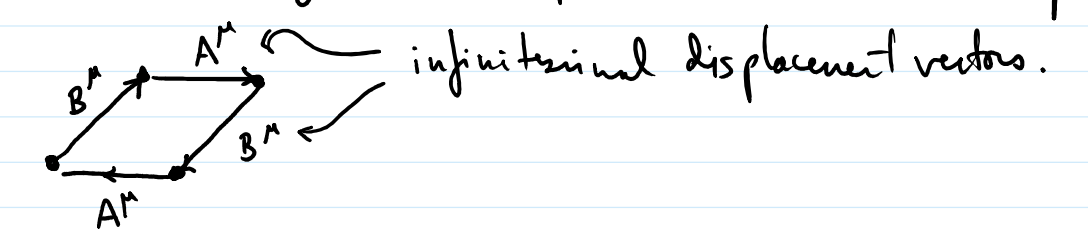
\includegraphics[width=15cm]{parallel-transport.png}
\end{figure}

We can ask ourselves the following question: how does the same vector change under the above process, i.e., under the displacement \( x^\mu \rightarrow x^\mu + B^\mu \). We would see that:
\begin{align*}
	v \rightarrow v^\mu + B^\alpha v_\alpha v^\mu + ... 
\end{align*}
If we add on the displacement, \( x^\mu + B^\mu \rightarrow x^\mu + B^\mu + A^\mu \), we see that: 
\begin{align*}
	 v^\mu + B^\alpha V_\alpha V^\mu \rightarrow V^\mu + B^\alpha V_\alpha V^\mu + A^\beta \nabla_\beta ( V^\mu + B^\alpha \nabla_\alpha V^\mu), 
\end{align*}
and so on...
\newline 
\newline
So if we transport around the entire loop, then \( V \) will change as: 
\begin{align}
	\delta V^p = A^\mu A^\nu [ \nabla_\mu, \nabla_\nu ] V^\rho = A^\mu B^\nu ( \nabla_\mu \nabla_\nu - \nabla_\nu \nabla_\mu ) V^\rho. 	
\end{align}
Note that covariant derivatives DO NOT commute. The above captures how vectors will change when you move around in small loops. This is a \textbf{characterization} of the local curvature at some point in space-time. We will define the \textbf{curvatue tensor/Riemann tensor} by:
\begin{align}
	\delta V^\rho = \tensor{R}{^\rho_{\sigma \mu \nu}}	 A^\mu B^\nu V^\sigma. 
\end{align}
This is a \( (1,3)\)-tensor, which by definition is going to be anti-symmetric in its last two indices thanks to the commutator. \( A \) and \( B \) are arbitrary vectors that we use to measure curvature in different directions. Let's compute \( \riemanntensor \):
\begin{align*}
	[ \nabla_\mu, \nabla_\nu ] v^\rho & = \nabla_\mu ( \nabla_\nu v^\rho) - \nabla_\nu ( \nabla_\mu v^\rho ) \\
	& = \partial_\mu ( \nabla_\nu v^\rho) - \tensor{\Gamma}{^\lambda_{\mu \nu}} \nabla_\lambda v^\rho + \tensor{\Gamma}{^\lambda_{\mu \nu}} + \tensor{\Gamma}{^\rho_{\mu \sigma}} \nabla_\nu v^\sigma - ( \mu \leftrightarrow \nu ) 
\end{align*}
Observe that the Christoffel symbols by definition are symmetric in its lower indices. We then obtain: 
\begin{align*}
	& = \partial_\mu ( \partial_\nu v^\rho ) - \partial_\mu ( \tensor{\Gamma}{^\mu_{\nu \sigma}} v^\sigma) + \tensor{\Gamma}{^\rho_{\mu \sigma}} \partial_\nu v^\sigma + \tensor{\Gamma}{^\rho_{\mu \sigma}} \tensor{\Gamma}{^\sigma_{\nu \lambda}} v^\lambda - ( \mu \leftrightarrow \nu ) \\
\end{align*}
By the equality of the mixed partials, the first two terms will cancel. We get, after re-labelling the indices \( \sigma \leftrightarrow \lambda \): 
\begin{align*}
	& = v^\sigma ( \partial_\mu \tensor{\Gamma}{^\partial_{\nu \sigma}} + \tensor{\Gamma}{^\rho_{\mu \lambda}} \tensor{\Gamma}{^\lambda_{\nu \lambda}} - ( \mu \leftrightarrow \nu ) ) \\
	& = \riemanntensor v^\sigma. 
\end{align*}
So, to summarize: 
\begin{align}
\boxed{\riemanntensor := \partial_\mu \tensor{\Gamma}{^\rho_{\nu \sigma}} - \partial_\nu \tensor{\Gamma}{^\rho_{\mu \sigma}} + \tensor{\Gamma}{^\rho_{\mu \lambda}} \tensor{\Gamma}{^\lambda_{\nu \sigma}} - \tensor{\Gamma}{^\rho_{\nu \lambda}} \tensor{\Gamma}{^\lambda_{\mu \sigma}}}	
\end{align}
Now we need to unpack and understand this expression for curvature. First we'll state some facts about the curvature tensor: 
\begin{enumerate}[noitemsep]
	\item \( \riemanntensor \) is a tensor even though \( \Gamma \) is not. 
	\item If \( \riemanntensor = 0 \) then we say that the space-time is \textbf{flat.}
	\item \textbf{Theorem.} space-time is flat \( \iff \) there is a coordinate system where the metric \( \grmetric \) is constant. The ``proof'': for the forward direction it follows from a complicated theorem that we will ignore; for the backward direction it follows easily since the Christoffel symbols vanish. 
\end{enumerate}
Now we'll define the following quantity by lowering the indices: 
\begin{align*}
	R_{\rho \sigma \mu \nu} := g_{\rho \alpha} \tensor{R}{^\alpha_{\sigma \mu \nu}}
\end{align*}
We have the following properties of this: 
\begin{enumerate}[noitemsep]
	\item (Anti-symmetric in the second pair of indices): \( R_{\rho \sigma \mu \nu} = - R_{\rho \sigma \nu \mu} \). 
	\item (Anti-symmetric in its first two indices): \(  R_{\rho \sigma \mu \nu} = - R_{\sigma \rho \mu \nu} \). 
	\item \(  R_{\rho \sigma \mu \nu} = R_{\mu \nu \rho \sigma} \).
	\item (Total symmetrization vanishes): \( R_{[\rho \sigma \mu \nu ]} = 0 \) (this is important).
\end{enumerate}
The Riemann tensor involves the first and second derivatives of the metric, but the important feature is it packages them into a tensor, so if the Riemann tensor vanishes in one coordinate system then it much vanish in \emph{every} coordinate system. However, we want something that's simpler than a four-index tensor. We ask ourselves the following question: \textbf{Q: What is the sort of thing we could construct from the Riemann tensor?} Let's contract the upper indices with a lower index to get the \textbf{Ricci tensor}:
\begin{align}
	R_{\mu \nu} := \tensor{R}{^\rho_{\mu \rho \nu}}.
\end{align}
By the symmetries of the Riemann tensor, this is the \emph{only} possible contraction. 
\begin{definition}[Ricci Tensor]
	\( R_{\mu \nu} := \tensor{R}{^\rho_{\mu \rho \nu}} \) is the \textbf{Ricci Tensor}, a \( (0,2) \)-tensor. This tensor is symmetric, and up to a sign is the only \( (0,2) \)-tensor formed by contracting the indices of the Riemann tensor. 
\end{definition}
We can use the metric to define something even simpler.
\begin{definition}[Ricci Scalar]
	We define the \textbf{Ricci Scalar} as:
	\begin{align}
		R := R_{\mu \nu} g^{\mu \nu}.	
	\end{align}
\end{definition}
Let's take a step back. We are developing a theorem of differential geometry to define the curvature of space-time. The equations of motion obeyed by space-time will be an equation involving the curvature (so the Riemann tensor). One possible equation that could describe the curvature of space-time is: 
\begin{align*}
	\riemanntensor = 0, 
\end{align*}
but this would describe flat space-time. This is too simple. Let's go to the next simplest one: 
\begin{align*}
	R_{\mu \nu} = 0.
\end{align*}
This is Einstein's equation in the \emph{absence} of matter!

\section{Lecture 11: 11 Feb 2021}

\end{document}
